\sectionframe{Results}

\begin{frame}{Inferring Age from Images}{IMDB-WIKI}
	\begin{table}[t]
		\setlength{\tabcolsep}{2.5pt}
		\small
		\begin{center}
			\resizebox{0.6\textwidth}{!}{
				\begin{tabular}{l|cccc|cccc}
					\toprule[1.5pt]
					Metrics      & \multicolumn{4}{c|}{MAE~$\downarrow$}     & \multicolumn{4}{c}{GM~$\downarrow$}  \\ \midrule
					Shot         & All  & Many & Med. & Few   & All  & Many & Med. & Few   \\ \midrule\midrule
					\textsc{Vanilla}      & 8.06 & 7.23 & 15.12  & 26.33 & 4.57 & 4.17 & 10.59  & 20.46 \\ \midrule\midrule
					\textsc{SmoteR}~(\cite{torgo2013smote})       & 8.14 & 7.42 & 14.15  & 25.28 & 4.64 & \textbf{4.30} & 9.05   & 19.46 \\[1.2pt]
					\textsc{SMOGN}~(\cite{branco2017smogn})        & 8.03 & \textbf{7.30} & 14.02  & 25.93 & 4.63 & \textbf{4.30} & 8.74   & 20.12 \\[1.2pt]
					\textsc{SMOGN} + \textbf{\textsc{LDS}}   & 8.02 & 7.39 & 13.71 & 23.22 & 4.63 & 4.39 & 8.71 & 15.80 \\[1.2pt]
					\textsc{SMOGN} + \textbf{\textsc{FDS}}   & 8.03 & 7.35 & 14.06 & 23.44 & 4.65 & 4.33 & 8.87 & 16.00 \\[1.2pt]
					\textsc{SMOGN} + \textbf{\textsc{LDS}} + \textbf{\textsc{FDS}}   & \textbf{7.97} & 7.38 & \textbf{13.22} & \textbf{22.95} & \textbf{4.59} & 4.39 & \textbf{7.84} & \textbf{14.94} \\ \midrule\midrule
					\textsc{Focal-R}      & 7.97 & 7.12 & 15.14  & 26.96 & 4.49 & 4.10 & 10.37  & 21.20 \\[1.2pt]
					\textsc{Focal-R} + \textbf{\textsc{LDS}} & {7.90}  & \textbf{7.10}  &  14.72   & 25.84  & \textbf{4.47}   & \textbf{4.09}    & {10.11}     & {19.14}     \\[1.2pt]
					\textsc{Focal-R} + \textbf{\textsc{FDS}}   & 7.96 & 7.14 & 14.71 & 26.06 & 4.51 & 4.12 & 10.16 & 19.56 \\[1.2pt]
					\textsc{Focal-R} + \textbf{\textsc{LDS}} + \textbf{\textsc{FDS}}   & \textbf{7.88} & \textbf{7.10} & \textbf{14.08}  & \textbf{25.75}   & \textbf{4.47} & 4.11 & \textbf{9.32} & \textbf{18.67} \\ \midrule\midrule
					\textsc{RRT}          & 7.81 & 7.07 & 14.06  & 25.13 & 4.35 & 4.03 & 8.91   & 16.96 \\[1.2pt]
					\textsc{RRT} + \textbf{\textsc{LDS}} & {7.79} &  7.08  & {13.76}  & {24.64} & {4.34} & \textbf{4.02} & {8.72} & {16.92} \\[1.2pt]
					\textsc{RRT} + \textbf{\textsc{FDS}}   & \textbf{7.65}  & \textbf{7.02} & 12.68 & 23.85 & \textbf{4.31} & 4.03 & 7.58 & 16.28 \\[1.2pt]
					\textsc{RRT} + \textbf{\textsc{LDS}} + \textbf{\textsc{FDS}}   & \textbf{7.65}  & 7.06  & \textbf{12.41}  & \textbf{23.51}  & \textbf{4.31} & {4.07} & \textbf{7.17} & \textbf{15.44} \\ \midrule\midrule
					\textsc{SQInv}      & 7.87 & 7.24 & 12.44  & 22.76 & 4.47 & 4.22 & 7.25   & 15.10 \\[1.2pt]
					\textsc{SQInv} + \textbf{\textsc{LDS}} & {7.83} & 7.31 & \textbf{12.43}  & {22.51} & {4.42} & {4.19} & {7.00}  & {13.94} \\[1.2pt]
					\textsc{SQInv} + \textbf{\textsc{FDS}}   & 7.83 & 7.23 & 12.60  & 22.37  & 4.42 & 4.20 & \textbf{6.93} & 13.48  \\[1.2pt]
					\textsc{SQInv} + \textbf{\textsc{LDS}} + \textbf{\textsc{FDS}}   & \textbf{7.78} & \textbf{7.20} & {12.61} & \textbf{22.19} & \textbf{4.37}    & \textbf{4.12} & 7.39  & \textbf{12.61}  \\ \midrule\midrule
					\textsc{\textbf{Ours~(best)} vs. Vanilla}   & \textcolor{darkgreen}{\textbf{+0.41}} & \textcolor{darkgreen}{\textbf{+0.21}} & \textcolor{darkgreen}{\textbf{+2.71}} & \textcolor{darkgreen}{\textbf{+4.14}} & \textcolor{darkgreen}{\textbf{+0.26}} & \textcolor{darkgreen}{\textbf{+0.15}} & \textcolor{darkgreen}{\textbf{+3.66}} & \textcolor{darkgreen}{\textbf{+7.85}} \\
					\bottomrule[1.5pt]
				\end{tabular}
			}
		\end{center}
	\end{table}
	\begin{itemize}\fontsize{7pt}{7.2}\selectfont
		\item Either LDS, FDS, or both leads to performance gains.
		\item LDS + FDS often achieves the best results:
		\begin{itemize}\fontsize{7pt}{7.2}\selectfont
			\item maintains or improves performance overall
			and on many-shot regions,
			\item boosts performance for medium-shot and few-shot regions.
		\end{itemize}
	\end{itemize}
	\credit{Table}{yang2021delving}
\end{frame}

\begin{frame}{Inferring Age from Images}{AgeDB}
	\begin{table}[t]
		\setlength{\tabcolsep}{2.5pt}
		\small
		\begin{center}
			\resizebox{0.6\textwidth}{!}{
				\begin{tabular}{l|cccc|cccc}
					\toprule[1.5pt]
					Metrics      & \multicolumn{4}{c|}{MAE~$\downarrow$}     & \multicolumn{4}{c}{GM~$\downarrow$}  \\ \midrule
					Shot         & All  & Many & Med. & Few   & All  & Many & Med. & Few   \\ \midrule\midrule
					\textsc{Vanilla}      & 7.77 & 6.62 & 9.55   & 13.67 & 5.05 & 4.23 & 7.01   & 10.75 \\ \midrule\midrule
					\textsc{SmoteR}~(\cite{torgo2013smote})       & 8.16  & 7.39   & 8.65 & 12.28 & 5.21    & 4.65    & 5.69 & 8.49    \\[1.2pt]
					\textsc{SMOGN}~(\cite{branco2017smogn})        & 8.26  & 7.64   & 9.01 & 12.09 & 5.36    & 4.90    & 6.19 & 8.44    \\[1.2pt]
					\textsc{SMOGN} + \textbf{\textsc{LDS}}   & 7.96 & 7.44 & 8.64  & 11.77 & 5.03 & 4.68 & 5.69  & 7.98  \\[1.2pt]
					\textsc{SMOGN} + \textbf{\textsc{FDS}}   & 8.06 & 7.52 & 8.75  & 11.89 & 5.02 & 4.66 & 5.63  & 8.02  \\[1.2pt]
					\textsc{SMOGN} + \textbf{\textsc{LDS}} + \textbf{\textsc{FDS}}   & \textbf{7.90} & \textbf{7.32}  & \textbf{8.51}  & \textbf{11.19}  & \textbf{4.98}  & \textbf{4.64}  & \textbf{5.41} & \textbf{7.35} \\ \midrule\midrule
					\textsc{Focal-R}      & 7.64 & 6.68 & 9.22   & 13.00 & 4.90 & 4.26 & 6.39   & 9.52  \\[1.2pt]
					\textsc{Focal-R} + \textbf{\textsc{LDS}}      & 7.56 & \textbf{6.67} & 8.82   & 12.40 & 4.82 & 4.27 & 5.87   & 8.83  \\[1.2pt]
					\textsc{Focal-R} + \textbf{\textsc{FDS}}      & 7.65 & 6.89 & 8.70   & \textbf{11.92} & 4.83 & 4.32 & 5.89   & \textbf{8.04}  \\[1.2pt]
					\textsc{Focal-R} + \textbf{\textsc{LDS}} + \textbf{\textsc{FDS}} & \textbf{7.47} & 6.69 & \textbf{8.30}  & 12.55 & \textbf{4.71} & \textbf{4.25} & \textbf{5.36}  & 8.59  \\ \midrule\midrule
					\textsc{RRT}          & 7.74 & 6.98 & 8.79   & 11.99 & 5.00 & 4.50 & 5.88   & 8.63  \\[1.2pt]
					\textsc{RRT} + \textbf{\textsc{LDS}}     & {7.72} & 7.00 & {8.75}   & {11.62} & {4.98} & 4.54 & {5.71}   & {8.27}  \\[1.2pt]
					\textsc{RRT} + \textbf{\textsc{FDS}}     & {7.70} & \textbf{6.95} & {8.76}   & {11.86} & {4.82} & \textbf{4.32} & {5.83}   & {8.08}  \\[1.2pt]
					\textsc{RRT} + \textbf{\textsc{LDS}} + \textbf{\textsc{FDS}}     & \textbf{7.66} & 6.99 & \textbf{8.60}   & \textbf{11.32} & \textbf{4.80} & 4.42 & \textbf{5.53}   & \textbf{6.99}  \\ \midrule\midrule
					\textsc{SQInv}      & 7.81 & 7.16 & 8.80   & 11.20 & 4.99 & 4.57 & 5.73   & 7.77  \\[1.2pt]
					\textsc{SQInv} + \textbf{\textsc{LDS}} & 7.67 & \textbf{6.98} & 8.86   & 10.89 & 4.85 & {4.39} &  5.80  & {7.45}  \\[1.2pt]
					\textsc{SQInv} + \textbf{\textsc{FDS}} & 7.69 & 7.10 & 8.86   & \textbf{9.98} & 4.83 & {4.41} &  5.97  & \textbf{6.29}  \\[1.2pt]
					\textsc{SQInv} + \textbf{\textsc{LDS}} + \textbf{\textsc{FDS}} & \textbf{7.55} &  7.01  & \textbf{8.24}   & 10.79 & \textbf{4.72} & \textbf{4.36} & \textbf{5.45}  & {6.79}  \\ \midrule\midrule
					\textsc{\textbf{Ours~(best)} vs. Vanilla}   & \textcolor{darkgreen}{\textbf{+0.30}} & \textcolor{lightblue}{\textbf{-0.05}} & \textcolor{darkgreen}{\textbf{+1.31}} & \textcolor{darkgreen}{\textbf{+3.69}} & \textcolor{darkgreen}{\textbf{+0.34}} & \textcolor{lightblue}{\textbf{-0.02}} & \textcolor{darkgreen}{\textbf{+1.65}} & \textcolor{darkgreen}{\textbf{+4.46}} \\
					\bottomrule[1.5pt]
				\end{tabular}
			}
		\end{center}
	\end{table}
	\begin{itemize}\fontsize{7pt}{7.2}\selectfont
		\item Either LDS, FDS, or both leads to performance gains.
		\item LDS + FDS often achieves the best results:
		\begin{itemize}\fontsize{7pt}{7.2}\selectfont
			\item maintains or improves performance overall
			and on many-shot regions,
			\item boosts performance for medium-shot and few-shot regions.
		\end{itemize}
	\end{itemize}
	\credit{Table}{yang2021delving}
\end{frame}

\begin{frame}{Inferring Text Similarity Score}{STS-B}
	\begin{table}[!htbp]
		\setlength{\tabcolsep}{2.5pt}
		\small
		\begin{center}
			\resizebox{0.6\textwidth}{!}{
				\begin{tabular}{l|cccc|cccc}
					\toprule[1.5pt]
					Metrics      & \multicolumn{4}{c|}{MSE~$\downarrow$}       & \multicolumn{4}{c}{Pearson correlation~(\%)~$\uparrow$}    \\ \midrule
					Shot         & All   & Many  & Med. & Few   & All   & Many  & Med. & Few   \\ \midrule\midrule
					\textsc{Vanilla}      & 0.974 & 0.851 & 1.520  & 0.984 & 74.2 & 72.0 & 62.7  & 75.2 \\ \midrule\midrule
					\textsc{SmoteR}~ (\cite{torgo2013smote})       & 1.046     & 0.924     & 1.542      & 1.154     & 72.6     & 69.3     & 65.3      & 70.6     \\[1.2pt]
					\textsc{SMOGN}~(\cite{branco2017smogn})        & 0.990     & 0.896     & 1.327      & 1.175     & 73.2     & 70.4     & 65.5      & 69.2     \\[1.2pt]
					\textsc{SMOGN} + \textbf{\textsc{LDS}}   & 0.962     & 0.880     & 1.242      & 1.155     & 74.0     & 71.5     & 65.2      & 69.8     \\[1.2pt]
					\textsc{SMOGN} + \textbf{\textsc{FDS}}   & 0.987    & 0.945    & \textbf{1.101}      & 1.153     & 73.0    & 69.6    & \textbf{68.5}      & 69.9     \\[1.2pt]
					\textsc{SMOGN} + \textbf{\textsc{LDS}} + \textbf{\textsc{FDS}}   &  \textbf{0.950}   & \textbf{0.851}    & 1.327      & \textbf{1.095}     & \textbf{74.6}    & \textbf{72.1}    & 65.9      & \textbf{71.7}     \\ \midrule\midrule
					\textsc{Focal-R}      & 0.951 & 0.843 & 1.425  & 0.957 & 74.6 & 72.3 & 61.8  & 76.4 \\[1.2pt]
					\textsc{Focal-R} + \textbf{\textsc{LDS}} & 0.930     & \textbf{0.807}     & 1.449      & 0.993     & \textbf{75.7}     & \textbf{73.9}     & 62.4      & 75.4 \\[1.2pt]
					\textsc{Focal-R} + \textbf{\textsc{FDS}} & \textbf{0.920} & 0.855 & \textbf{1.169}  & 1.008     & 75.1     & 72.6   & \textbf{66.4}      & 74.7 \\[1.2pt]
					\textsc{Focal-R} + \textbf{\textsc{LDS}} + \textbf{\textsc{FDS}} & 0.940 & 0.849 & 1.358  & \textbf{0.916}     & 74.9     & 72.2     & 66.3      & \textbf{77.3} \\ \midrule\midrule
					\textsc{RRT}         & 0.964 & 0.842 & 1.503  & 0.978 & 74.5 & 72.4 & 62.3  & 75.4 \\[1.2pt]
					\textsc{RRT} + \textbf{\textsc{LDS}}     & {0.916} & 0.817 & {1.344}  & 0.945 & {75.7} & {73.5} & {64.1}  & {76.6} \\[1.2pt]
					\textsc{RRT} + \textbf{\textsc{FDS}} & 0.929 & 0.857 & \textbf{1.209}  & 1.025     & 74.9     & 72.1     & \textbf{67.2}      & 74.0 \\[1.2pt]
					\textsc{RRT} + \textbf{\textsc{LDS}} + \textbf{\textsc{FDS}} & \textbf{0.903} & \textbf{0.806} & 1.323  & \textbf{0.936}     & \textbf{76.0}     &\textbf{73.8}     & 65.2      & \textbf{76.7} \\ \midrule\midrule
					\textsc{Inv}      & 1.005 & 0.894 & 1.482  & 1.046 & 72.8 & 70.3 & 62.5  & 73.2 \\[1.2pt]
					\textsc{Inv} + \textbf{\textsc{LDS}} & 0.914 & 0.819 & {1.319}  & {0.955} & {75.6} & {73.4} & {63.8}  & {76.2} \\[1.2pt]
					\textsc{Inv} + \textbf{\textsc{FDS}} & 0.927 & 0.851 & \textbf{1.225}  & 1.012     & 75.0     & 72.4     & \textbf{66.6}      & 74.2 \\[1.2pt]
					\textsc{Inv} + \textbf{\textsc{LDS}} + \textbf{\textsc{FDS}} & \textbf{0.907} & \textbf{0.802} & 1.363  & \textbf{0.942}     & \textbf{76.0}     & \textbf{74.0}     & 65.2      & \textbf{76.6} \\ \midrule\midrule
					\textsc{\textbf{Ours~(best)} vs. Vanilla}   & \textcolor{darkgreen}{\textbf{+.071}} & \textcolor{darkgreen}{\textbf{+.049}} & \textcolor{darkgreen}{\textbf{+.419}} & \textcolor{darkgreen}{\textbf{+.068}} & \textcolor{darkgreen}{\textbf{+1.8}} & \textcolor{darkgreen}{\textbf{+2.0}} & \textcolor{darkgreen}{\textbf{+5.8}} & \textcolor{darkgreen}{\textbf{+2.1}} \\
					\bottomrule[1.5pt]
				\end{tabular}
			}
		\end{center}
	\end{table}
	\begin{itemize}
		\item Both LDS and FDS improve results for various methods, esp. medium- and few-shot regions.
	\end{itemize}
	\credit{Table}{yang2021delving}
\end{frame}

\begin{frame}{Inferring Depth}{NYUD2}
	\begin{table}[!t]
		\setlength{\tabcolsep}{2.5pt}
		\small
		\begin{center}
			\resizebox{0.7\textwidth}{!}{
				\begin{tabular}{l|cccc|cccc}
					\toprule[1.5pt]
					Metrics      & \multicolumn{4}{c|}{RMSE~$\downarrow$}       & \multicolumn{4}{c}{$\delta_1$~$\uparrow$}    \\ \midrule
					Shot         & All   & Many  & Med. & Few   & All   &Many   & Med. & Few   \\ \midrule\midrule
					\textsc{Vanilla}      & 1.477 & 0.591 & 0.952  & 2.123 & 0.677 & 0.777 &  0.693  & 0.570 \\ \midrule\midrule
					\textsc{Vanilla} + \textbf{\textsc{LDS}} &  1.387 &  0.671  &    0.913 & 1.954  & 0.672  & 0.701  & 0.706 & 0.630 \\[1.2pt]
					\textsc{Vanilla} + \textbf{\textsc{FDS}} & 1.442 & \textbf{0.615} & 0.940  & 2.059  & 0.681  & \textbf{0.760} & 0.695 & 0.596 \\[1.2pt]
					\textsc{Vanilla} + \textbf{\textsc{LDS}} + \textbf{\textsc{FDS}} & \textbf{1.338} & 0.670  & \textbf{0.851} & \textbf{1.880}  & \textbf{0.705} & 0.730  & \textbf{0.764}  & \textbf{0.655}  \\ \midrule\midrule
					\textsc{\textbf{Ours~(best)} vs. Vanilla}   & \textcolor{darkgreen}{\textbf{+.139}} & \textcolor{lightblue}{\textbf{-.024}} & \textcolor{darkgreen}{\textbf{+.101}} & \textcolor{darkgreen}{\textbf{+.243}} & \textcolor{darkgreen}{\textbf{+.028}} & \textcolor{lightblue}{\textbf{-.017}} & \textcolor{darkgreen}{\textbf{+.071}} & \textcolor{darkgreen}{\textbf{+.085}} \\
					\bottomrule[1.5pt]
				\end{tabular}
			}
		\end{center}
	\end{table}
	FDS and LDS
	\begin{itemize}
		\item alleviates overfitting on many-shot regions,
		\item generalizes better to all regions,
		\item slightly degrades many-shot region,
		\item boosts other regions.
	\end{itemize}
	\credit{Table}{yang2021delving}
\end{frame}

\begin{frame}{Inferring Health Score}{SHHS-DIR}
	\begin{table}[tb]
		\setlength{\tabcolsep}{2.5pt}
		\small
		\begin{center}
			\resizebox{0.7\textwidth}{!}{
				\begin{tabular}{l|cccc|cccc}
					\toprule[1.5pt]
					Metrics      & \multicolumn{4}{c|}{MAE~$\downarrow$}       & \multicolumn{4}{c}{GM~$\downarrow$}    \\ \midrule
					Shot         & All   & Many  & Med. & Few   & All   & Many  & Med. & Few   \\ \midrule\midrule
					\textsc{Vanilla}      & 15.36 & 12.47 & 13.98  & 16.94 & 10.63 & 8.04 &  9.59  & 12.20 \\ \midrule\midrule
					\textsc{Focal-R}      & 14.67 & 11.70  & 13.69  & 17.06 & 9.98 & 7.93 & 8.85 & 11.95 \\[1.2pt]
					\textsc{Focal-R} + \textbf{\textsc{LDS}} & 14.49  & 12.01  & 12.43 & 16.57 & 9.98 & 7.89 & 8.59 & 11.40  \\[1.2pt]
					\textsc{Focal-R} + \textbf{\textsc{FDS}} & 14.18 &  \textbf{11.06}  & 13.56 & 15.99 & 9.45 & \textbf{6.95} & 8.81 & 11.13 \\[1.2pt]
					\textsc{Focal-R} + \textbf{\textsc{LDS}} + \textbf{\textsc{FDS}} & \textbf{14.02} & 11.08 &  \textbf{12.24} & \textbf{15.49}  & \textbf{9.32} & 7.18  & \textbf{8.10}  & \textbf{10.39}  \\ \midrule\midrule
					\textsc{RRT}         & 14.78 & 12.43 & 14.01 & 16.48 & 10.12 & 8.05 & 9.71 & 11.96 \\[1.2pt]
					\textsc{RRT} + \textbf{\textsc{LDS}}     & {14.56} & 12.08 & {13.44}  & 16.45 & {9.89} & {7.85} & {9.18}  & {11.82} \\[1.2pt]
					\textsc{RRT} + \textbf{\textsc{FDS}} & 14.36 & 11.97 & {13.33}  & 16.08 & 9.74 & 7.54 & 9.20  & 11.31 \\[1.2pt]
					\textsc{RRT} + \textbf{\textsc{LDS}} + \textbf{\textsc{FDS}} & \textbf{14.33} & \textbf{11.96} & \textbf{12.47}  & \textbf{15.92}     & \textbf{9.63}     & \textbf{7.35}     & \textbf{8.74} & \textbf{11.17} \\ \midrule\midrule
					\textsc{Inv}      & 14.39 & 11.84 & 13.12  & 16.02 & 9.34 & 7.73 & 8.49  & 11.20 \\[1.2pt]
					\textsc{Inv} + \textbf{\textsc{LDS}} & 14.14 & 11.66 & {12.77}  & {16.05} & {9.26} & {7.64} & {8.18}  & {11.32} \\[1.2pt]
					\textsc{Inv} + \textbf{\textsc{FDS}} & 13.91 & \textbf{11.12} & {12.29}  & 15.53 & 8.94  & \textbf{6.91}  & {7.79}      & 10.65 \\[1.2pt]
					\textsc{Inv} + \textbf{\textsc{LDS}} + \textbf{\textsc{FDS}} & \textbf{13.76} & \textbf{11.12} & \textbf{12.18}  & \textbf{15.07}     & \textbf{8.70}     & 6.94     & \textbf{7.60}      & \textbf{10.18} \\ \midrule\midrule
					\textsc{\textbf{Ours~(best)} vs. Vanilla}   & \textcolor{darkgreen}{\textbf{+1.60}} & \textcolor{darkgreen}{\textbf{+1.41}} & \textcolor{darkgreen}{\textbf{+1.80}} & \textcolor{darkgreen}{\textbf{+1.87}} & \textcolor{darkgreen}{\textbf{+1.93}} & \textcolor{darkgreen}{\textbf{+1.13}} & \textcolor{darkgreen}{\textbf{+1.99}} & \textcolor{darkgreen}{\textbf{+2.02}} \\
					\bottomrule[1.5pt]
				\end{tabular}
			}
		\end{center}
	\end{table}
	\begin{itemize}
		\item Both FDS and LDS are effective.
		\item FDS + LDS often get highest gains over all tested regions.
		\item Note: SMOTER and SMOGN not directly applicable.
	\end{itemize}
	\credit{Table}{yang2021delving}
\end{frame}

%\begin{frame}{Extrapolation \& Interpolation}
%\end{frame}
%
%\begin{frame}{Understanding FDS}
%\end{frame}

\begin{frame}{Ablation: kernel type}{IMDB-WIKI}
	\begin{table}[tb]
		\setlength{\tabcolsep}{7.5pt}
		\begin{center}
			\small
			\resizebox{0.95\textwidth}{!}{
				\begin{tabular}{l|cccc|cccc|cccc}
					\toprule[1.5pt]
					Metrics      &\multicolumn{4}{c|}{MSE~$\downarrow$} & \multicolumn{4}{c|}{MAE~$\downarrow$}       & \multicolumn{4}{c}{GM~$\downarrow$}    \\ \midrule
					Shot         & All   & Many  & Med. & Few & All   & Many  & Med. & Few   & All   & Many  & Med. & Few   \\ \midrule\midrule
					\textsc{Vanilla}   & 138.06 &  108.70  & 366.09  & 964.92  & 8.06 & 7.23 & 15.12  & 26.33 & 4.57 & 4.17 & 10.59  & 20.46 \\ \midrule\midrule
					\multicolumn{9}{l}{\emph{\textbf{LDS:}}} \\ \midrule
					\textsc{Gaussian Kernel}   & 131.65 & 109.04 & 298.98 & 834.08  & {7.83} & 7.31 & {12.43}  & {22.51} & {4.42} & {4.19} & {7.00}  & {13.94} \\[1.2pt]
					\textsc{Triangular Kernel} & 133.77 & 110.24  & 309.70 & 850.74 & 7.89 & 7.30 & 12.72 & 22.80 & 4.50 & 4.24 & 7.75 & 14.91  \\[1.2pt]
					\textsc{Laplacian Kernel} & 132.87 &  109.27  & 312.10 & 829.83 & 7.87 & 7.29 & 12.68 & 22.38 & 4.50 & 4.26 & 7.29 & 13.71\\ \midrule\midrule
					\multicolumn{9}{l}{\emph{\textbf{FDS:}}} \\ \midrule
					\textsc{Gaussian Kernel}      & 133.81 & 107.51 & 332.90 & 916.18 & 7.85 & 7.18 & 13.35 & 24.12 & 4.47 & 4.18 & 8.18 & 15.18 \\[1.2pt]
					\textsc{Triangular Kernel} & 134.09 & 110.49 & 301.18 & 927.99 & 7.97 & 7.41 & 12.20 & 23.99 & 4.64 & 4.41 & 7.06 & 14.28  \\[1.2pt]
					\textsc{Laplacian Kernel} & 133.00 & 104.26 & 352.95 & 968.62 & 8.05 & 7.25 & 14.78 & 26.16 & 4.71 & 4.33 & 10.19 & 19.09 \\
					\bottomrule[1.5pt]
				\end{tabular}
			}
		\end{center}
	\end{table}
	\begin{itemize}
		\item All kernel types lead to gains
		\item Often best results with Gaussian kernel
	\end{itemize}
	\credit{Table}{yang2021delving}
\end{frame}

\begin{frame}{Ablation: kernel type}{STS-B}
	\begin{table}[tb]
		\setlength{\tabcolsep}{4pt}
		\begin{center}
			\small
			\resizebox{0.95\textwidth}{!}{
				\begin{tabular}{l|cccc|cccc|cccc|cccc}
					\toprule[1.5pt]
					Metrics      &\multicolumn{4}{c|}{MSE~$\downarrow$} & \multicolumn{4}{c|}{MAE~$\downarrow$}       & \multicolumn{4}{c|}{Pearson correlation (\%)~$\uparrow$} & \multicolumn{4}{c}{Spearman correlation (\%)~$\uparrow$}   \\ \midrule
					Shot         & All   & Many  & Med. & Few & All   & Many  & Med. & Few    & All   & Many  & Med. & Few & All   & Many  & Med. & Few   \\ \midrule\midrule
					\textsc{Vanilla}   & 0.974 & 0.851 & 1.520 & 0.984 & 0.794 & 0.740 & 1.043 & 0.771 & 74.2 & 72.0 & 62.7 & 75.2 & 74.4 & 68.8 & 50.5 & 75.0 \\ \midrule\midrule
					\multicolumn{9}{l}{\emph{\textbf{LDS:}}} \\ \midrule
					\textsc{Gaussian Kernel}   & 0.914 & 0.819 & 1.319 & 0.955 & 0.773 & 0.729 & 0.970 & 0.772  & 75.6 & 73.4 & 63.8 & 76.2 & 76.1 &  70.4 & 55.6 & 74.3 \\[1.2pt]
					\textsc{Triangular Kernel} & 0.938 & 0.870 & 1.193 & 1.039 & 0.786 & 0.754 & 0.929 & 0.784  & 74.8 & 72.4 & 64.1 & 74.0 & 75.2 & 69.3 & 54.1 & 73.9  \\[1.2pt]
					\textsc{Laplacian Kernel} & 0.938 & 0.829 & 1.413 & 0.962 & 0.782 & 0.731 & 1.014 & 0.773 & 75.7 & 73.0 & 65.8 & 76.5 & 76.0 & 70.0 & 52.3 & 75.2 \\ \midrule\midrule
					\multicolumn{9}{l}{\emph{\textbf{FDS:}}} \\ \midrule
					\textsc{Gaussian Kernel}      & 0.916 & 0.875 & 1.027 & 1.086 & 0.767 & 0.746 & 0.840 & 0.811  & 75.5 & 73.0 & 67.0 & 72.8 & 75.8 & 69.9 & 54.4 & 72.0  \\[1.2pt]
					\textsc{Triangular Kernel} & 0.935 & 0.863 & 1.239 & 0.966 & 0.762 & 0.725 & 0.912 & 0.788 & 74.6 & 72.4 & 64.8 & 75.9 & 74.4 & 69.1 & 48.4 & 75.4  \\[1.2pt]
					\textsc{Laplacian Kernel} & 0.925 & 0.843 & 1.247 & 1.020 & 0.771 & 0.733 & 0.929 & 0.800 & 75.0 & 72.6 & 64.7 & 74.2 & 75.4 & 70.1 & 53.5 & 73.5  \\
					\bottomrule[1.5pt]
				\end{tabular}
			}
		\end{center}
	\end{table}
	\begin{itemize}
		\item All kernel types lead to gains
		\item Often best results with Gaussian kernel
	\end{itemize}
	\credit{Table}{yang2021delving}
\end{frame}

\begin{frame}{Ablation: Gaussian kernel hyper-parameters}{IMDB-WIKI}
	\vspace{-1.3em}
	\begin{table}[tb]
		\setlength{\tabcolsep}{7.5pt}
		\begin{center}
			\small
			\resizebox{0.65\textwidth}{!}{
				\begin{tabular}{c|c|cccc|cccc|cccc}
					\toprule[1.5pt]
					\multicolumn{2}{l|}{Metrics}      &\multicolumn{4}{c|}{MSE~$\downarrow$} & \multicolumn{4}{c|}{MAE~$\downarrow$}       & \multicolumn{4}{c}{GM~$\downarrow$}    \\ \midrule
					\multicolumn{2}{l|}{Shot}         & All   & Many  & Med. & Few & All   & Many  & Med. & Few   & All   & Many  & Med. & Few   \\ \midrule\midrule
					\multicolumn{2}{l|}{\textsc{Vanilla}}   & 138.06 &  108.70  & 366.09  & 964.92  & 8.06 & 7.23 & 15.12  & 26.33 & 4.57 & 4.17 & 10.59  & 20.46 \\ \midrule\midrule
					$l$ & $\sigma$ &  \\ \midrule\midrule
					\multicolumn{9}{l}{\emph{\textbf{LDS:}}} \\ \midrule
					\texttt{5}&\texttt{1}   & 132.08 & 108.53 & 309.03 & 843.53   & 7.80 & 7.22 & 12.61 & 22.33 &4.42 & 4.19 & 7.16 & 12.54 \\[1.2pt]
					\texttt{9}&\texttt{1} & 135.04 & 112.32 & 307.90 & 803.15   & 7.97 & 7.39 & 12.74 & 22.19 & 4.55 & 4.30 & 7.53 & 14.11  \\[1.2pt]
					\texttt{15}&\texttt{1} & 134.06 & 110.49 & 308.83 &  864.30 & 7.84 & 7.28 & 12.35 & 22.81 & 4.44 & 4.22 & 6.95 & 14.22\\[1.2pt] 
					\texttt{5}&\texttt{2}   & 131.65 & 109.04 & 298.98 & 834.08  & 7.83 & 7.31 & 12.43  & 22.51 & 4.42 & 4.19 & 7.00  & 13.94 \\[1.2pt]
					\texttt{9}&\texttt{2} & 136.78 & 112.41 & 322.65 & 850.47   & 8.02 & 7.41 & 13.00 & 23.23 & 4.55 & 4.29 & 7.55 & 15.65  \\[1.2pt]
					\texttt{15}&\texttt{2} & 135.66 & 111.68 & 319.20 & 833.02   & 7.98 & 7.40 & 12.74 & 22.27 & 4.60 & 4.37 & 7.30 & 12.92\\[1.2pt] 
					\texttt{5}&\texttt{3}   & 137.56 & 113.50 & 322.47 & 831.38 & 8.07 & 7.47 & 13.06 & 22.85 & 4.63 & 4.36 & 7.87 & 15.11 \\[1.2pt]
					\texttt{9}&\texttt{3} & 138.91 & 114.89 & 319.40 & 863.16   & 8.18 & 7.57 & 13.19 & 23.33 & 4.71 & 4.44 & 8.09 & 15.17  \\[1.2pt]
					\texttt{15}&\texttt{3} & 138.86 & 114.25 & 326.97 & 856.27   & 8.18 & 7.54 & 13.53 & 23.17 & 4.77 & 4.47 & 8.52 & 15.25\\ \midrule\midrule
					\multicolumn{9}{l}{\emph{\textbf{FDS:}}} \\ \midrule
					% $l$ & $\sigma$ &  \\ \midrule
					\texttt{5}&\texttt{1}   & 133.63 & 104.80 & 354.24 & 972.54 & 7.87 & 7.06 & 14.71 & 25.96 & 4.42 & 4.04 & 9.95 & 18.47 \\[1.2pt]
					\texttt{9}&\texttt{1} & 134.34 & 105.97 & 356.54 & 919.16 & 7.95 & 7.18 & 14.58 & 24.80 & 4.54 & 4.20 & 9.56 & 15.13  \\[1.2pt]
					\texttt{15}&\texttt{1} & 136.32 & 107.47 & 355.84 & 948.71 & 7.97 & 7.23 & 14.81 & 25.59 & 4.60 & 4.23 & 9.99 & 17.60 \\[1.2pt]
					\texttt{5}&\texttt{2}   & 133.81 & 107.51 & 332.90 & 916.18 & 7.85 & 7.18 & 13.35 & 24.12 & 4.47 & 4.18 & 8.18 & 15.18 \\[1.2pt]
					\texttt{9}&\texttt{2} & 133.99 & 105.01 & 357.31 & 963.79 & 7.94 & 7.11 & 14.95 & 25.97 & 4.48 & 4.09 & 10.49 & 18.19  \\[1.2pt]
					\texttt{15}&\texttt{2} & 136.61 & 107.93 & 361.08 & 973.56 & 7.98 & 7.23 & 14.68 & 25.21 & 4.61 & 4.24 & 10.14 & 17.91 \\[1.2pt] 
					\texttt{5}&\texttt{3}   & 136.81 & 107.76 & 359.08 & 953.16 & 7.98 & 7.18 & 14.85 & 24.94 & 4.53 & 4.15 & 10.27 & 17.33 \\[1.2pt]
					\texttt{9}&\texttt{3} & 133.48 & 104.14 & 359.80 & 972.29 & 7.94 & 7.09 & 15.04 & 25.87 & 4.48 & 4.09 & 10.40 & 16.85  \\[1.2pt]
					\texttt{15}&\texttt{3} & 132.55 & 103.08 & 360.39 & 970.43 & 8.03 & 7.22 & 14.86 & 25.40 & 4.67 & 4.33 & 10.04 & 13.86 \\
					\bottomrule[1.5pt]
				\end{tabular}
			}
		\end{center}
	\end{table}
	\begin{itemize}\tiny
		\item Gaussian kernel size $l\in\{5,9,15\}$ and standard deviation $\sigma\in\{1,2,3\}$
		\item LDS
		\vskip-1ex
		\begin{itemize}\tiny
			%\item $11.4\%$ to $15.7\%$ relative MAE improvements in few-shot regions.
			\item Smaller $\sigma$ usually leads to slightly better results over all regions. 
			\item Larger gains w.r.t. the performance in medium-shot and few-shot regions.
			\item Minor degradation in many-shot regions.
		\end{itemize}
		\item FDS
		\vskip-1ex
		\begin{itemize}\tiny
			\item Smaller $l$ often obtains slightly higher improvements over all regions.
			\item Equally boosts all the regions, with slightly smaller improvements in medium-shot and few-shot regions.
		\end{itemize}
		\item $3.3$-$6.2\%$ overall MSE gain
		\item Best results with $l=5$ and $\sigma=2$
		\item Robust to different hyper-parameters
	\end{itemize}
	\credit{Table}{yang2021delving}
\end{frame}

\begin{frame}{Ablation: Gaussian kernel hyper-parameters}{STS-B}
	\begin{table}[H]
		\setlength{\tabcolsep}{6pt}
		\begin{center}
			\small
			\resizebox{0.79\textwidth}{!}{
				\begin{tabular}{c|c|cccc|cccc|cccc|cccc}
					\toprule[1.5pt]
					\multicolumn{2}{l|}{Metrics}      &\multicolumn{4}{c|}{MSE~$\downarrow$} & \multicolumn{4}{c|}{MAE~$\downarrow$}       & \multicolumn{4}{c|}{Pearson correlation (\%)~$\uparrow$} & \multicolumn{4}{c}{Spearman correlation (\%)~$\uparrow$}   \\ \midrule
					\multicolumn{2}{l|}{Shot}   & All   & Many  & Med. & Few   & All   & Many  & Med. & Few & All   & Many  & Med. & Few & All   & Many  & Med. & Few   \\ \midrule\midrule
					\multicolumn{2}{l|}{\textsc{Vanilla}}   & 0.974 & 0.851 & 1.520 & 0.984 & 0.794 & 0.740 & 1.043 & 0.771  & 74.2 & 72.0 & 62.7 & 75.2 & 74.4 & 68.8 & 50.5 & 75.0 \\ \midrule\midrule
					$l$ & $\sigma$ &  \\ \midrule\midrule
					\multicolumn{9}{l}{\emph{\textbf{LDS:}}} \\ \midrule
					\texttt{5}&\texttt{1}   & 0.942 & 0.825 & 1.431 & 1.023 & 0.781 & 0.726 & 1.016 & 0.809 & 75.1 & 73.2 & 61.8 & 74.5 & 75.3 & 70.2 & 52.2 & 72.5 \\[1.2pt]
					\texttt{9}&\texttt{1} & 0.931 & 0.840 & 1.323 & 0.962 & 0.785 & 0.744 & 0.972 & 0.773 & 75.0 & 72.7 & 63.3 & 75.8 & 75.6 & 70.1 & 53.6 & 74.8  \\[1.2pt]
					\texttt{15}&\texttt{1} & 0.941 & 0.833 & 1.413 & 0.953 & 0.781 & 0.728 & 1.014 & 0.776 & 75.0 & 72.8 & 62.6 & 76.3 & 75.5 & 70.2 & 52.0 & 74.6 \\[1.2pt] 
					\texttt{5}&\texttt{2}   & 0.914 & 0.819 & 1.319 & 0.955 & 0.773 & 0.729 & 0.970 & 0.772 & 75.6 & 73.4 & 63.8 & 76.2 & 76.1 &  70.4 & 55.6 & 74.3 \\[1.2pt]
					\texttt{9}&\texttt{2} & 0.926 & 0.823 & 1.379 & 0.944 & 0.782 & 0.733 & 1.003 & 0.764 & 75.5 & 73.4 & 63.6 & 76.8 & 76.0 & 70.5 & 53.5 & 76.2  \\[1.2pt]
					\texttt{15}&\texttt{2} & 0.949 & 0.831 & 1.452 & 1.005 & 0.788 & 0.735 & 1.023 & 0.782 & 74.9 & 72.9 & 63.0 & 74.7 & 75.4 & 70.1 & 52.5 & 73.6 \\[1.2pt]
					\texttt{5}&\texttt{3}   & 0.928 & 0.845 & 1.250 & 1.041 & 0.775 & 0.733 & 0.951 & 0.798 & 75.1 & 73.3 & 63.2 & 73.8 & 75.3 & 70.4 & 51.4 & 72.6 \\[1.2pt]
					\texttt{9}&\texttt{3} & 0.939 & 0.816 & 1.462 & 1.000 & 0.786 & 0.732 & 1.030 & 0.783 & 75.3 & 73.5 & 62.6 & 74.7 & 75.9 & 70.9 & 53.0 & 73.7  \\[1.2pt]
					\texttt{15}&\texttt{3} & 0.927 & 0.824 & 1.348 & 1.010 & 0.774 & 0.726 & 0.982 & 0.780 & 75.2 & 73.4 & 62.2 & 74.6 & 75.7 & 70.7 & 53.0 & 72.3 \\ \midrule\midrule
					\multicolumn{9}{l}{\emph{\textbf{FDS:}}} \\ \midrule
					% $l$ & $\sigma$ &  \\ \midrule
					\texttt{5}&\texttt{1}   & 0.943 & 0.869 & 1.217 & 1.066 & 0.776 & 0.742 & 0.914 & 0.799 & 74.4 & 71.7 & 65.6 & 72.5 & 74.2 & 68.4 & 51.1 & 71.2 \\[1.2pt]
					\texttt{9}&\texttt{1} & 0.927 & 0.851 & 1.193 & 1.096 & 0.770 & 0.736 & 0.896 & 0.822 & 74.9 & 72.8 & 65.8 & 71.6 & 74.8 & 69.7 & 52.3 & 68.3  \\[1.2pt]
					\texttt{15}&\texttt{1} & 0.926 & 0.854 & 1.202 & 1.029 & 0.776 & 0.743 & 0.914 & 0.800 & 74.9 & 72.6 & 66.1 & 74.0 & 75.1 & 69.8 & 49.5 & 73.6 \\[1.2pt] 
					\texttt{5}&\texttt{2}   & 0.916 & 0.875 & 1.027 & 1.086 & 0.767 & 0.746 & 0.840 & 0.811 & 75.5 & 73.0 & 67.0 & 72.8 & 75.8 & 69.9 & 54.4 & 72.0 \\[1.2pt]
					\texttt{9}&\texttt{2} & 0.933 & 0.888 & 1.068 & 1.081 & 0.776 & 0.752 & 0.855 & 0.839 & 74.8 & 72.0 & 67.9 & 72.2 & 74.9 & 68.9 & 53.3 & 72.0  \\[1.2pt]
					\texttt{15}&\texttt{2} & 0.944 & 0.890 & 1.125 & 1.078 & 0.783 & 0.761 & 0.864 & 0.822 & 74.4 & 71.8 & 65.8 & 72.2 & 74.5 & 68.9 & 53.1 & 70.9 \\[1.2pt]
					\texttt{5}&\texttt{3}   & 0.924 & 0.860 & 1.190 & 0.964 & 0.771 & 0.740 & 0.897 & 0.790 & 75.0 & 72.7 & 64.4 & 76.1 & 75.1 & 69.4 & 53.8 & 76.5 \\[1.2pt]
					\texttt{9}&\texttt{3} & 0.932 & 0.878 & 1.149 & 0.982 & 0.770 & 0.746 & 0.876 & 0.780 & 74.8 & 72.5 & 63.8 & 75.3 & 74.8 & 69.3 & 50.2 & 75.6  \\[1.2pt]
					\texttt{15}&\texttt{3} & 0.956 & 0.915 & 1.110 & 1.016 & 0.784 & 0.767 & 0.855 & 0.803 & 74.4 & 72.1 & 63.7 & 75.5 & 74.3 & 68.7 & 50.0 & 74.6 \\
					\bottomrule[1.5pt]
				\end{tabular}
			}
		\end{center}
	\end{table}
	\begin{itemize}
		\item Gaussian kernel size $l\in\{5,9,15\}$ and standard deviation $\sigma\in\{1,2,3\}$
		\item $3.3$-$6.2\%$ overall MSE gain
		\item Best results with $l=5$ and $\sigma=2$
		\item Robust to different hyper-parameters
	\end{itemize}
	\credit{Table}{yang2021delving}
\end{frame}

\begin{frame}{Ablation: loss function}{STS-B}
	\vspace{-1.8cm}
	\begin{table}[H]
		\setlength{\tabcolsep}{5pt}
		\begin{center}
			\small
			\resizebox{0.95\textwidth}{!}{
				\begin{tabular}{l|cccc|cccc|cccc|cccc}
					\toprule[1.5pt]
					Metrics      &\multicolumn{4}{c|}{MSE~$\downarrow$} & \multicolumn{4}{c|}{MAE~$\downarrow$}       &  \multicolumn{4}{c|}{Pearson correlation (\%)~$\uparrow$} & \multicolumn{4}{c}{Spearman correlation (\%)~$\uparrow$}   \\ \midrule
					Shot         & All   & Many  & Med. & Few   & All   & Many  & Med. & Few & All   & Many  & Med. & Few & All   & Many  & Med. & Few   \\ \midrule\midrule
					\multicolumn{9}{l}{\emph{\textbf{LDS:}}} \\ \midrule
					\textsc{MAE (L1)}   & 0.893 & 0.808 & 1.241 & 0.964 & 0.765 & 0.727 & 0.938 & 0.758 & 76.3 & 73.9 & 66.0 & 75.9 & 76.7 & 71.1 & 54.5 & 75.6 \\[1.2pt]
					\textsc{MSE (L2)} & 0.914 & 0.819 & 1.319 & 0.955 & 0.773 & 0.729 & 0.970 & 0.772  & 75.6 & 73.4 & 63.8 & 76.2 & 76.1 &  70.4 & 55.6 & 74.3  \\[1.2pt]
					\textsc{Huber Loss (sL1)} & 0.902 & 0.811 & 1.276 & 0.978 & 0.761 & 0.718 & 0.954 & 0.751 & 76.1 & 74.2 & 64.7 & 75.5 & 76.5 & 71.6 & 52.9 & 74.3 \\ \midrule\midrule
					\multicolumn{9}{l}{\emph{\textbf{FDS:}}} \\ \midrule
					\textsc{MAE (L1)}    & 0.918 & 0.860 & 1.105 & 1.082 & 0.762 & 0.733 & 0.859 & 0.833 & 75.5 & 73.7 & 65.3 & 72.3 & 75.6 & 70.9 & 52.1 & 71.5    \\[1.2pt]
					\textsc{MSE (L2)}  & 0.916 & 0.875 & 1.027 & 1.086 & 0.767 & 0.746 & 0.840 & 0.811  & 75.5 & 73.0 & 67.0 & 72.8 & 75.8 & 69.9 & 54.4 & 72.0  \\[1.2pt]
					\textsc{Huber Loss (sL1)} & 0.920 & 0.867 & 1.097 & 1.052 & 0.765 & 0.741 & 0.858 & 0.800 & 75.3 & 72.9 & 66.6 & 73.6 & 75.3 & 69.7 & 52.3 & 73.6  \\
					\bottomrule[1.5pt]
				\end{tabular}
			}
		\end{center}
	\end{table}
	\begin{itemize}
		\item Similar results for all losses
		\item Robust to different losses
	\end{itemize}
	\begin{tikzpicture}[remember picture, overlay]
		\node[above=7em,left=1em] at (current page.south east) 
		{
			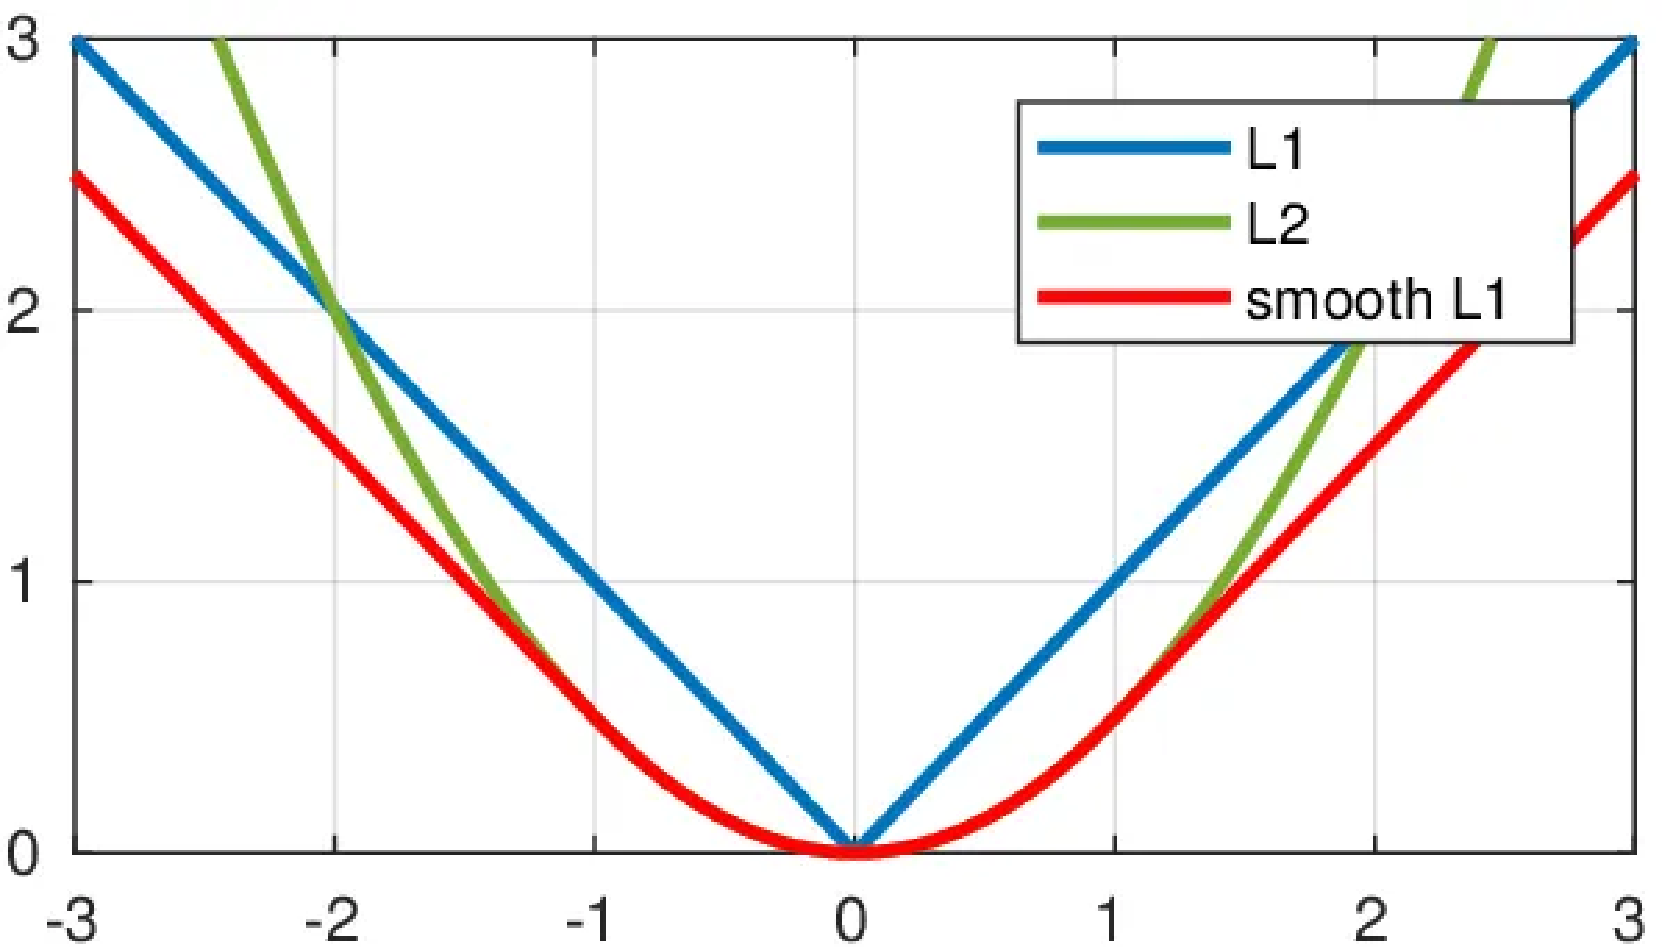
\includegraphics[width=0.5\textwidth]{images/losses.pdf}
		};
	\end{tikzpicture}
	\footlineextra{%
		\creditbase{Table}{yang2021delving}, \crediturlbase{Image}{https://medium.com/artificialis/loss-functions-361b2ad439a}%
	}
\end{frame}

%\begin{frame}{Ablation: robustness to diverse skewed label densities}
%\end{frame}

\begin{frame}{Could LDS + FDS help when label distribution is skewed with one or more Gaussian peaks?}
	\begin{itemize}\setlength\itemsep{1.5em}
		\item Experimental setup
		\begin{itemize}
			\item Curated skewed label distributions with 1-4 Gaussian peaks on IMDB-WIKI-DIR
			\item Compared to vanilla model
		\end{itemize}
	\end{itemize}
\end{frame}

\begin{frame}{Skewed label distribution with one Gaussian peak}{IMDB-WIKI}
	\begin{figure}[h]
		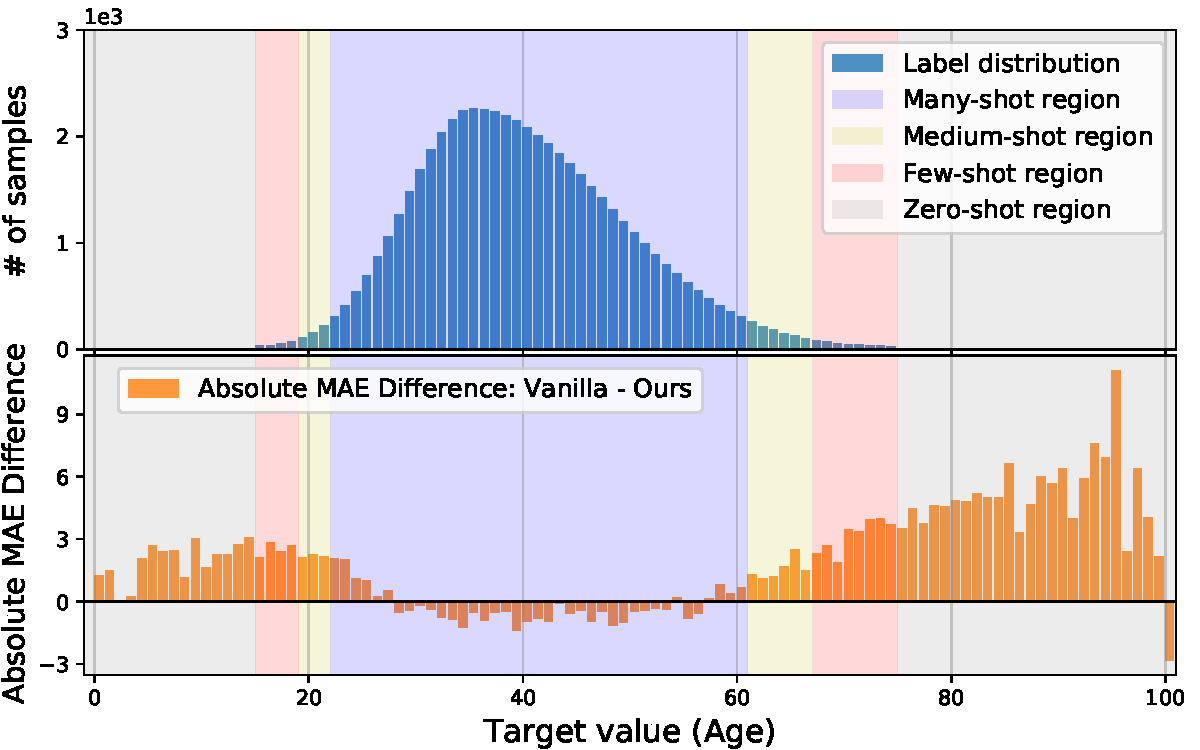
\includegraphics[width=0.7\linewidth]{images/interp_extrap_diff_peak1.pdf}
		\caption{MAE gains of LDS + FDS over vanilla model.}
	\end{figure}
	\begin{itemize}
		\item Performance gains, esp. for extrapolation \& interpolation
	\end{itemize}
	\credit{Image}{yang2021delving}
\end{frame}

\begin{frame}{Skewed label distribution with two Gaussian peaks}{IMDB-WIKI}
	\begin{figure}[h]
		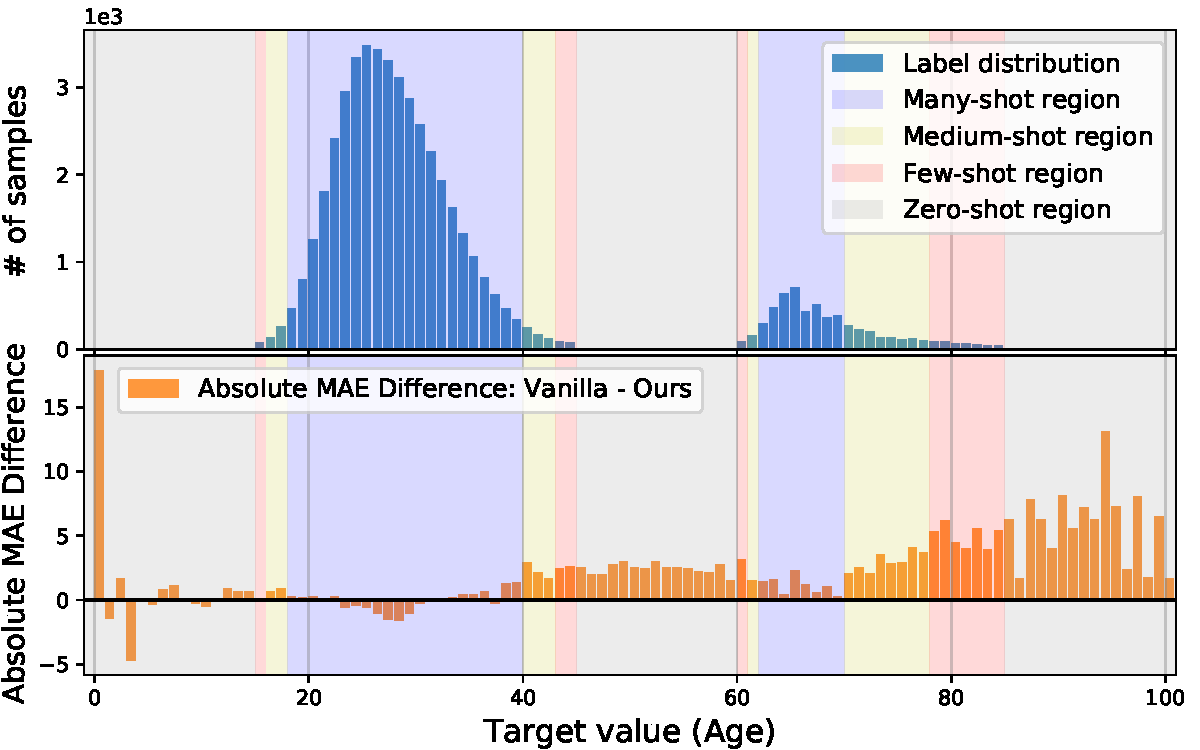
\includegraphics[width=0.7\linewidth]{images/interp_extrap_diff_peak2.pdf}
		\caption{MAE gains of LDS + FDS over vanilla model.}
	\end{figure}
	\begin{itemize}
		\item Performance gains, esp. for extrapolation \& interpolation
	\end{itemize}
	\credit{Image}{yang2021delving}
\end{frame}

\begin{frame}{Skewed label distribution with three Gaussian peaks}{IMDB-WIKI}
	\begin{figure}[h]
		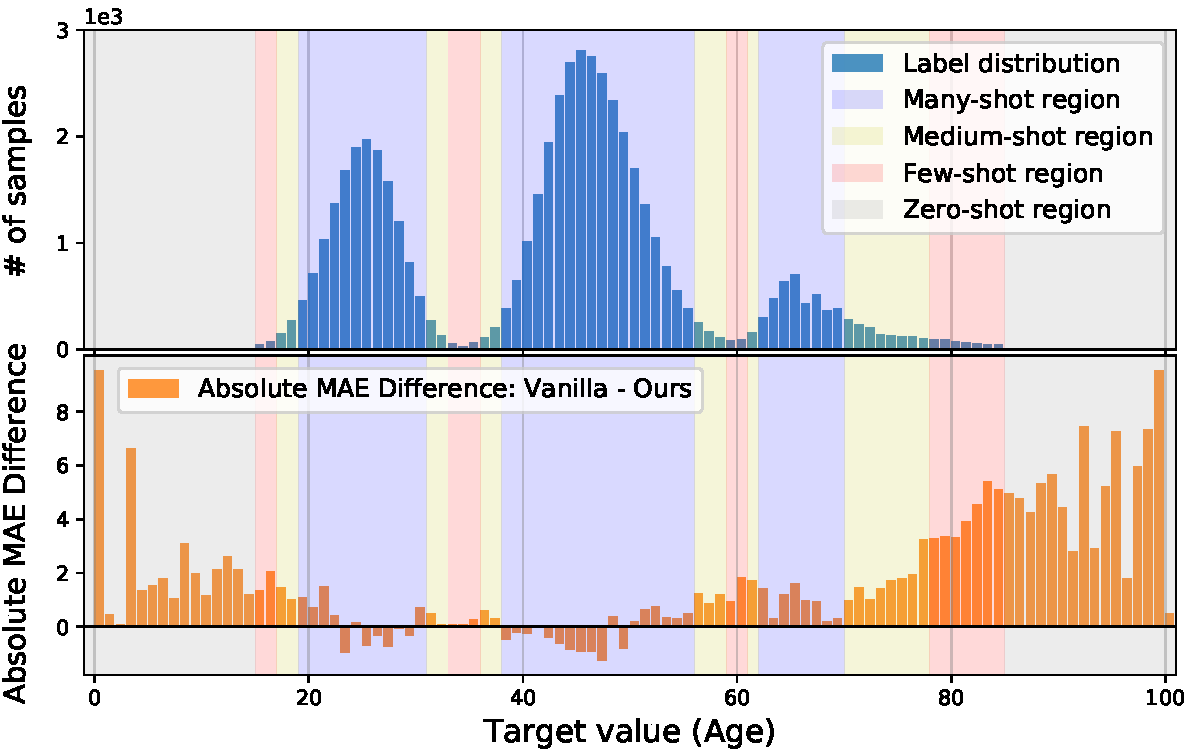
\includegraphics[width=0.7\linewidth]{images/interp_extrap_diff_peak3.pdf}
		\caption{MAE gains of LDS + FDS over vanilla model.}
	\end{figure}
	\begin{itemize}
		\item Performance gains, esp. for extrapolation \& interpolation
	\end{itemize}
	\credit{Image}{yang2021delving}
\end{frame}

\begin{frame}{Skewed label distribution with four Gaussian peaks}{IMDB-WIKI}
	\begin{figure}[h]
		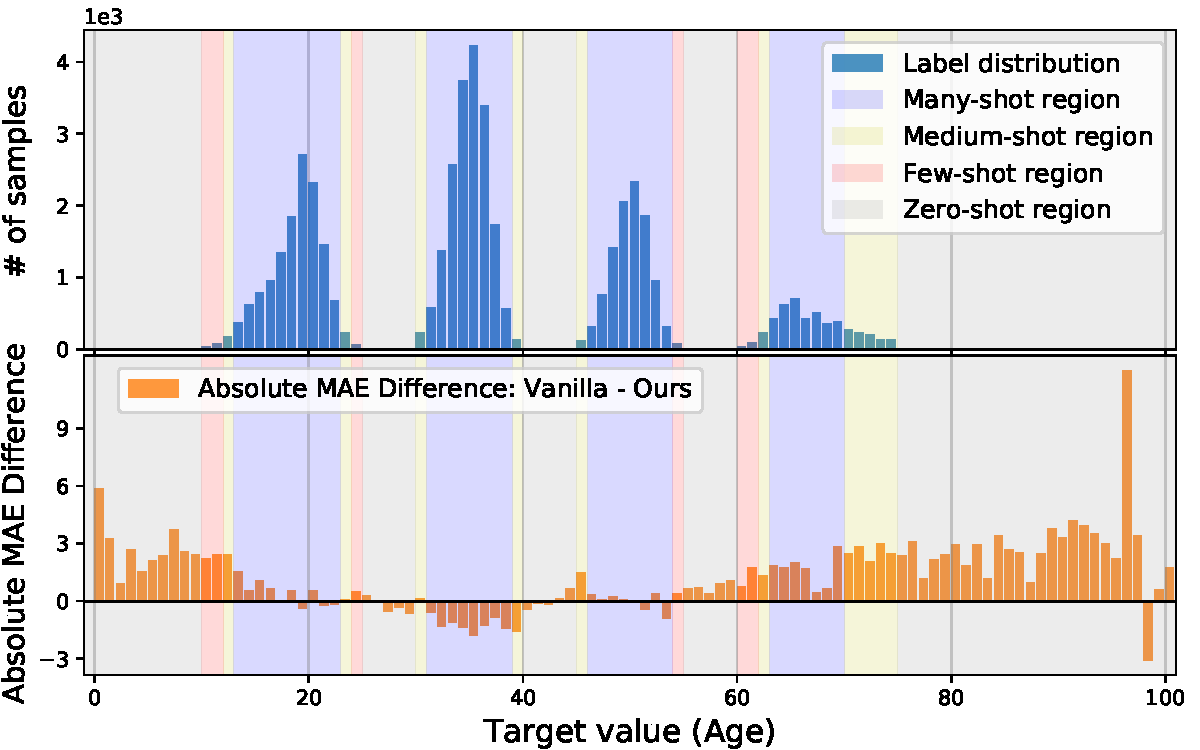
\includegraphics[width=0.7\linewidth]{images/interp_extrap_diff_peak4.pdf}
		\caption{MAE gains of LDS + FDS over vanilla model.}
	\end{figure}
	\begin{itemize}
		\item Performance gains, esp. for extrapolation \& interpolation
	\end{itemize}
	\credit{Image}{yang2021delving}
\end{frame}

\begin{frame}{Could LDS + FDS help when label distribution is skewed with one or more Gaussian peaks?}
	\begin{itemize}\setlength\itemsep{1.5em}
		\item Experimental setup
		\begin{itemize}
			\item Curated skewed label distributions with 1-4 Gaussian peaks on IMDB-WIKI-DIR
			\item Compared to vanilla model
		\end{itemize}
		\item Findings
		\begin{itemize}
			\item Robustness to distribution change
			\item Brings improvement
		\end{itemize}
	\end{itemize}
\end{frame}

%\begin{frame}{Skewed label distribution with two Gaussian peaks}{IMDB-WIKI}
%	\begin{table}[t]
%		\setlength{\tabcolsep}{1.5pt}
%		\small
%		\begin{center}
%			\resizebox{\textwidth}{!}{
%				\begin{tabular}{l|cccc|cccc}
%					\toprule[1.5pt]
%					Metrics      & \multicolumn{4}{c|}{MAE~$\downarrow$}       & \multicolumn{4}{c}{GM~$\downarrow$}    \\ \midrule
%					Shot         & All   & w/ data  & Interp. & Extrap.   & All   & w/ data  & Interp. & Extrap.   \\ \midrule\midrule
%					\textsc{Vanilla}      & 11.72 & 9.32 & 16.13  & 18.19 & 7.44 & 5.33 &  14.41  & 16.74 \\ \midrule\midrule
%					\textsc{Vanilla} + \textbf{\textsc{LDS}} &  10.54 &  8.31  &    14.14 & 17.38  & 6.50  & 4.67  & 12.13 & 15.36 \\[1.2pt]
%					\textsc{Vanilla} + \textbf{\textsc{FDS}} & 11.40 & 8.97 & 15.83  & 18.01  & 7.18  & 5.12 & 14.02 & 16.48 \\[1.2pt]
%					\textsc{Vanilla} + \textbf{\textsc{LDS}} + \textbf{\textsc{FDS}} & \textbf{10.27} & \textbf{8.11}  & \textbf{13.71} & \textbf{17.02}  & \textbf{6.33} & \textbf{4.55}  & \textbf{11.71}  & \textbf{15.13}  \\ \midrule\midrule
%					\textsc{\textbf{Ours~(best)} vs. Vanilla}   & \textcolor{darkgreen}{\textbf{+1.45}} & \textcolor{darkgreen}{\textbf{+1.21}} & \textcolor{darkgreen}{\textbf{+2.42}} & \textcolor{darkgreen}{\textbf{+1.17}} & \textcolor{darkgreen}{\textbf{+1.11}} & \textcolor{darkgreen}{\textbf{+0.78}} & \textcolor{darkgreen}{\textbf{+2.70}} & \textcolor{darkgreen}{\textbf{+1.61}} \\
%					\bottomrule[1.5pt]
%				\end{tabular}
%			}
%		\end{center}
%		\caption{Interpolation \& extrapolation results}
%	\end{table}
%	\begin{itemize}
%		\item Best results by smoothing both label \& feature distributions
%	\end{itemize}
%	\credit{Table}{yang2021delving}
%\end{frame}

\begin{frame}{Different skewed label distributions}{IMDB-WIKI}
	\begin{table}[t]
		\setlength{\tabcolsep}{4.5pt}
		\label{table:appendix-skewed-dist}
		\small
		\begin{center}
			\resizebox{0.95\textwidth}{!}{
				\begin{tabular}{l|ccccccc|ccccccc}
					\toprule[1.5pt]
					Metrics      & \multicolumn{7}{c|}{MAE~$\downarrow$}       & \multicolumn{7}{c}{GM~$\downarrow$}    \\ \midrule
					Shot         & All   & Many & Med. & Few & Zero & Interp. & Extrap.   & All   & Many & Med. & Few & Zero & Interp. & Extrap.   \\ \midrule\midrule
					\multicolumn{9}{l}{\emph{\textbf{1 peak:}}} \\ \midrule
					\textsc{Vanilla}       & 11.20 & 6.05 & 11.43 & 14.76 & 22.67 & $-$ & 22.67 & 7.02 & \textbf{3.84} & 8.67 & 12.26 & 21.07 & $-$ & 21.07 \\ [1.2pt]
					\textsc{Vanilla} + \textbf{\textsc{LDS}}  & 10.09 & 6.26 & 9.91 & 12.12 & 19.37 & $-$ & 19.37 & 6.14 & 3.92 & 6.50 & 8.30 & 16.35 & $-$ & 16.35 \\[1.2pt]
					\textsc{Vanilla} + \textbf{\textsc{FDS}}  & 11.04 & \textbf{5.97} & 11.19 & 14.54 & 22.35 & $-$ & 22.35 & 6.96 & \textbf{3.84} & 8.54 & 12.08 & 20.71 & $-$ & 20.71 \\[1.2pt]
					\textsc{Vanilla} + \textbf{\textsc{LDS}} + \textbf{\textsc{FDS}}  & \textbf{10.00} & 6.28 & \textbf{9.66} & \textbf{11.83} & \textbf{19.21} & $-$ & \textbf{19.21} & \textbf{6.09} & 3.96 & \textbf{6.26} & \textbf{8.14} & \textbf{15.89} & $-$ & \textbf{15.89}  \\ \midrule\midrule
					\multicolumn{9}{l}{\emph{\textbf{2 peaks:}}} \\ \midrule
					\textsc{Vanilla}      & 11.72 & 6.83 & 11.78 & 15.35 & 16.86 & 16.13  & 18.19 & 7.44 & 3.61 & 8.06 & 12.94 &15.21&  14.41  & 16.74 \\ [1.2pt]
					\textsc{Vanilla} + \textbf{\textsc{LDS}} &  10.54  & 6.72 & 9.65 & 12.60 & 15.30&   14.14 & 17.38  & 6.50    & 3.65 & \textbf{5.65} & 9.30 & 13.20 & 12.13 & 15.36 \\[1.2pt]
					\textsc{Vanilla} + \textbf{\textsc{FDS}} & 11.40  & 6.69 & 11.02 & 14.85 & 16.61 & 15.83  & 18.01  & 7.18   & \textbf{3.50} & 7.49 & 12.73 & 14.86 & 14.02 & 16.48 \\[1.2pt]
					\textsc{Vanilla} + \textbf{\textsc{LDS}} + \textbf{\textsc{FDS}} & \textbf{10.27}  & \textbf{6.61} & \textbf{9.46} & \textbf{11.96} & \textbf{14.89} & \textbf{13.71} & \textbf{17.02}  & \textbf{6.33}   & 3.54 & 5.68 & \textbf{8.80} & \textbf{12.83} & \textbf{11.71}  & \textbf{15.13}  \\ \midrule\midrule
					\multicolumn{9}{l}{\emph{\textbf{3 peaks:}}} \\ \midrule
					\textsc{Vanilla}      & 9.83  & 7.01 & 9.81 & 11.93 & 20.11 & $-$ & 20.11 & 6.04 & 3.93 & 6.94 & 9.84 & 17.77 & $-$ & 17.77 \\ [1.2pt]
					\textsc{Vanilla} + \textbf{\textsc{LDS}} & 9.08 & \textbf{6.77} & 8.82 & 10.48 & 18.43 & $-$ & 18.43 & \textbf{5.35} & \textbf{3.78} & 5.63 & 7.49 & 15.46 & $-$ & 15.46 \\[1.2pt]
					\textsc{Vanilla} + \textbf{\textsc{FDS}} & 9.65 & 6.88 & 9.58 & 11.75 & 19.80 & $-$ & 19.80 & 5.86 & 3.83 & 6.68 & 9.48 & 17.43 & $-$ & 17.43 \\[1.2pt]
					\textsc{Vanilla} + \textbf{\textsc{LDS}} + \textbf{\textsc{FDS}} & \textbf{8.96} & 6.88 & \textbf{8.62} & \textbf{10.08} & \textbf{17.76} & $-$ & \textbf{17.76} & 5.38  & 3.90 & \textbf{5.61} & \textbf{7.36} & \textbf{14.65} & $-$ & \textbf{14.65}  \\ \midrule\midrule
					\multicolumn{9}{l}{\emph{\textbf{4 peaks:}}} \\ \midrule
					\textsc{Vanilla}      & 9.49 & 7.23 & 9.73 & 10.85 & 12.16 & 8.23 & 18.78 & 5.68 & 3.45 & 6.95 & 8.20 & 9.43 & 6.89 & 16.02 \\ [1.2pt]
					\textsc{Vanilla} + \textbf{\textsc{LDS}} & 8.80 & \textbf{6.98} & 8.26 & 10.07 & 11.26 & 8.31 & \textbf{16.22} & 5.10 & \textbf{3.33} & \textbf{5.07} & 7.08 & 8.47 & 6.66 & \textbf{12.74} \\[1.2pt]
					\textsc{Vanilla} + \textbf{\textsc{FDS}} & 9.28 & 7.11 & 9.16 & 10.88 & 11.95 & 8.30 & 18.11 & 5.49 & 3.36 & 6.35 & 8.15 & 9.21 & 6.82 & 15.30 \\[1.2pt]
					\textsc{Vanilla} + \textbf{\textsc{LDS}} + \textbf{\textsc{FDS}} & \textbf{8.76} & 7.07 & \textbf{8.23} & \textbf{9.54} & \textbf{11.13} & \textbf{8.05} & 16.32 & \textbf{5.05} & 3.36 & \textbf{5.07} & \textbf{6.56} & \textbf{8.30} & \textbf{6.34} & 13.10  \\ 
					\bottomrule[1.5pt]
				\end{tabular}
			}
		\end{center}
	\end{table}
	\begin{itemize}\fontsize{7pt}{7.2}\selectfont\setlength\itemsep{.5em}
		\item Typically best overall results by LDS + FDS
		\item Typically best many-shot results by LDS
		\item LDS + FDS can degrade many-shot region
	\end{itemize}
	\credit{Table}{yang2021delving}
\end{frame}


\begin{frame}{Balanced vs. Imbalanced Test Label Distribution}{IMDB-WIKI}
	\vspace{-0.2cm}
	\begin{table}[ht]
		\setlength{\tabcolsep}{6.5pt}
		\small
		\begin{center}
			\resizebox{0.95\textwidth}{!}{
				\begin{tabular}{l|cccc|cccc|cccc}
					\toprule[1.5pt]
					Metrics      & \multicolumn{4}{c|}{MSE~$\downarrow$}       & \multicolumn{4}{c|}{MAE~$\downarrow$}       & \multicolumn{4}{c}{GM~$\downarrow$}    \\ \midrule
					Shot         & All & Many & Med. & Few & All & Many & Med. & Few & All & Many & Med. & Few \\ \midrule\midrule
					\multicolumn{9}{l}{\emph{\textbf{Balanced:}}} \\ \midrule
					\textsc{Vanilla} & 138.06 & 108.70 & 366.09 & 964.92 & 8.06 & 7.23 & 15.12 & 26.33 & 4.57 & 4.17 & 10.59 & 20.46 \\ [1.2pt]
					\textsc{Vanilla} + \textbf{\textsc{LDS}} + \textbf{\textsc{FDS}} & \textbf{129.35} & \textbf{106.52} & \textbf{311.49} & \textbf{811.82} & \textbf{7.78} & \textbf{7.20} & \textbf{12.61} & \textbf{22.19} & \textbf{4.37} & \textbf{4.12} & \textbf{7.39}  & \textbf{12.61}  \\ \midrule\midrule
					\multicolumn{9}{l}{\emph{\textbf{Same as training set:}}} \\ \midrule
					\textsc{Vanilla} & \textbf{68.44} & \textbf{62.10} & 320.52 & 1350.01 & \textbf{5.84} & \textbf{5.72} & 15.11 & 30.54 & \textbf{3.44} & \textbf{3.40} & 11.76 & 24.06 \\ [1.2pt]
					\textsc{Vanilla} + \textbf{\textsc{LDS}} + \textbf{\textsc{FDS}} & 69.86 & 63.43 & \textbf{161.97} & \textbf{1067.89} & {5.90} & {5.77} & \textbf{9.94}  & \textbf{25.17} & {3.48} & {3.44} & \textbf{7.03} & \textbf{15.95} \\
					\bottomrule[1.5pt]
				\end{tabular}
			}
		\end{center}
	\end{table}
	\begin{itemize}
		\item Skewed label distribution for training set
		\item Case: balanced label distribution for test set.
		\begin{itemize}
			\item LDS and FDS can improve performance of all regions.
		\end{itemize}
		\item Case: skewed label distribution for test set, 
		\\same label distribution for training set.
		\begin{itemize}
			\item Minor degradation in many-shot region.
			\item Boosts in medium-shot and few-shot regions.
			\item Note: overall performance dominated by many-shot region, potentially biased and undesired evaluation.
		\end{itemize}
	\end{itemize}
	\credit{Table}{yang2021delving}
\end{frame}

\begin{frame}{Comparison to imbalanced classification methods}
	\vspace{-0.1cm}
	\begin{table}[ht]
		\setlength{\tabcolsep}{7pt}
		\small
		\begin{center}
			\resizebox{0.95\textwidth}{!}{
				\begin{tabular}{l|cccc|cccc|cccc}
					\toprule[1.5pt]
					Dataset & \multicolumn{4}{c|}{IMDB-WIKI-DIR (subsampled)} & \multicolumn{4}{c|}{STS-B-DIR} & \multicolumn{4}{c}{NYUD2-DIR} \\ \midrule
					Metric & \multicolumn{4}{c|}{MAE~$\downarrow$} & \multicolumn{4}{c|}{MSE~$\downarrow$} & \multicolumn{4}{c}{RMSE~$\downarrow$} \\ \midrule
					Shot & All & Many & Med. & Few & All & Many & Med. & Few & All & Many & Med. & Few \\ \midrule\midrule
					\multicolumn{9}{l}{\emph{\textbf{Imbalanced Classification:}}} \\ \midrule
					\textsc{Cls-vanilla} & 15.94 & 15.64 & 18.95 & 30.21 & 1.926 & 1.906 & 2.022 & 1.907 & 1.576 & 0.596 & 1.011 & 2.275 \\ [1.2pt]
					\textsc{CB}~(\cite{cui2019class}) & 22.41 & 22.32 & 22.05 & 32.90 & 2.159 & 2.194 & 2.028 & 2.107 & 1.664 & 0.592 & 1.044 & 2.415 \\ [1.2pt]
					\textsc{cRT}~(\cite{kang2019decoupling}) & 15.65 & 15.33 & 17.52 & 29.54 & 1.891 & 1.906 & 1.930 & 1.650 & 1.488 & 0.659 & 1.032 & 2.107 \\ \midrule\midrule
					\multicolumn{9}{l}{\emph{\textbf{Imbalanced Regression:}}} \\ \midrule
					\textsc{Reg-vanilla} & 14.64 & 13.98 & 17.47 & 30.29 & 0.974 & 0.851 & 1.520 & 0.984 & 1.477 & \textbf{0.591} & 0.952 & 2.123 \\ [1.2pt]
					\textsc{LDS} & {14.03} & {13.72} & {15.93} & {26.71} & 0.914 & 0.819 & 1.319 & 0.955 & 1.387 & 0.671 & 0.913 & 1.954 \\ [1.2pt]
					\textsc{FDS} & {13.97} & {13.55} & {16.42} & {24.64} & 0.916 & 0.875 & \textbf{1.027} & 1.086 & 1.442 & 0.615 & 0.940 & 2.059 \\ [1.2pt]
					\textsc{LDS + FDS} & \textbf{13.32} & \textbf{13.14} & \textbf{15.06} & \textbf{23.87} & \textbf{0.907} & \textbf{0.802} & 1.363 & \textbf{0.942} & \textbf{1.338} & 0.670 & \textbf{0.851} & \textbf{1.880} \\
					\bottomrule[1.5pt]
				\end{tabular}
			}
		\end{center}
	\end{table}
	\begin{itemize}\setlength\itemsep{.5em}\footnotesize
		\item Imbalanced regression methods outperform classification ones.
		\item Can reduce error up to 50-60\% in few-shot regions
		\item Imbalanced classification methods can perform worse than vanilla regression.
		\item Main finding: imbalance regression requires something different than just imbalance classification methods, which
		\begin{itemize}\setlength\itemsep{.1em}\footnotesize
			\item can ignore similarity between nearby targets,
			\item can ignore similarity between features linked to nearby targets,
			\item cannot interpolate \& extrapolate in continuous label space, so cannot deal with zero-shot label regions.
		\end{itemize}
	\end{itemize}
	\credit{Table}{yang2021delving}
\end{frame}